\documentclass[11pt]{article}
\usepackage{hyperref}
\usepackage{amsthm}
\usepackage{amsmath}
\usepackage{amsfonts}
\usepackage{tikz}
\usepackage{ wasysym }
\usepackage{fancyvrb}
\usetikzlibrary{arrows.meta,positioning}


\newtheorem{example}{Example}


\author{Group 1:  Nicholas Jacob}
\title{Homework 4 Advanced Analytics and Metaheuristics}

\begin{document}
\maketitle

\begin{enumerate}
\item Titan
\begin{enumerate}

\item Formulate the LP

Here is the model file for this section

{\tiny \VerbatimInput{group1_HW4_p1ai.mod}}

And here is the small data file

{\tiny \VerbatimInput{group1_HW4_p1ai.dat}}

\begin{enumerate}
\item We see the maximum return as \$1845200.  This includes a risk of 165900 units.  You will invest in $A$ the entire million.  You will take the profits in year 2 and hold in an account.  Then in year 3 all monies (million from $A$ and the cash held over from previous year) will be invested in $E$.

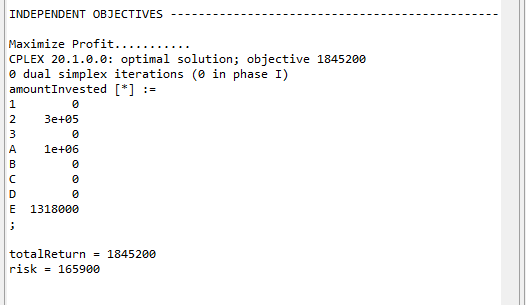
\includegraphics[width = .9\textwidth]{output1ai.png}

\item When minimizing risk, we do indeed see Mr. Lee's assumption come true, all monies are held in the bank.  They do gain compound interest...  Risk is 0 units and return is \$1191020

 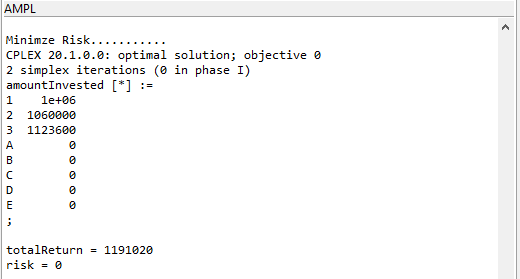
\includegraphics[width = .9\textwidth]{output1aii.png}

\item We preform the scalarization with $\gamma_1$ effecting the weight of the return and $\gamma_2$ effecting the weight of the risk.  We see the minimum risk ($\gamma_1 = 0$)at the top and the maximum return ($\gamma_1 = 1$) at the bottom.  Interestingly, we see that maximum return is generated at $\gamma_1 = \frac12$.  This is possibly due to the unbalanced range of the two objectives.  We note that return will vary from $[1191016,1845200]$ while risk varies from $[0,1659000]$.  Risk has about 2.5 times more range than return.

 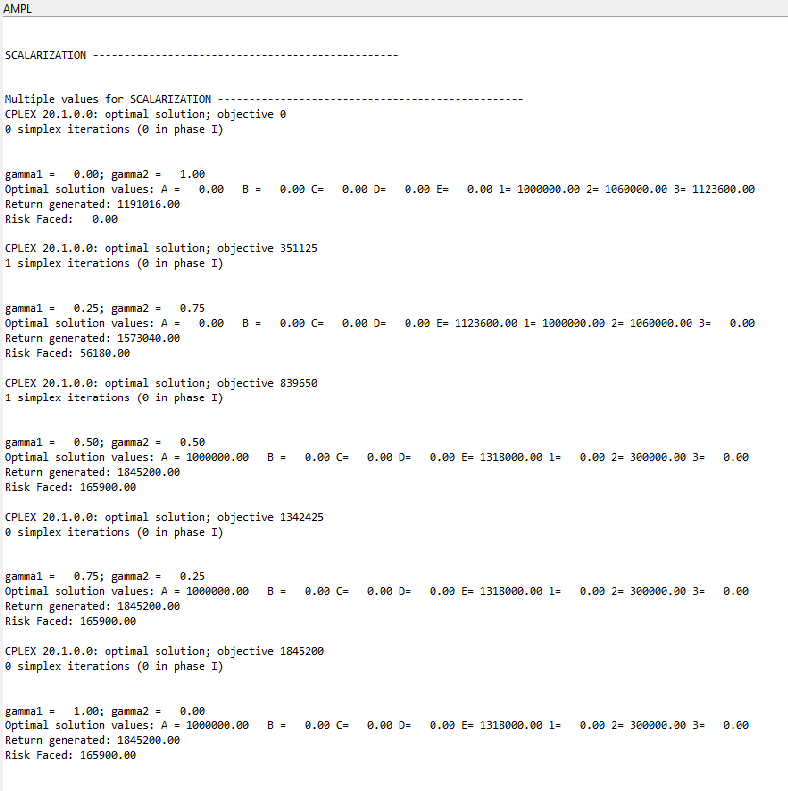
\includegraphics[width = .9\textwidth]{output1aiii.png}

We include the text output generated from this exercise for completeness.

{\tiny \VerbatimInput{titanParetoS.txt}}

\item Lastly, we preform $\epsilon$-constraint on this problem with 20 steps.  We use the risk as the constraint, setting
\[
\epsilon =\frac{episode\cdot maxRisk}{20}.
\]

We note that the minimum of the risk was zero so not included in the equation above.  We do not include all the 21 episodes of the output for brevity's sake but some are included below


 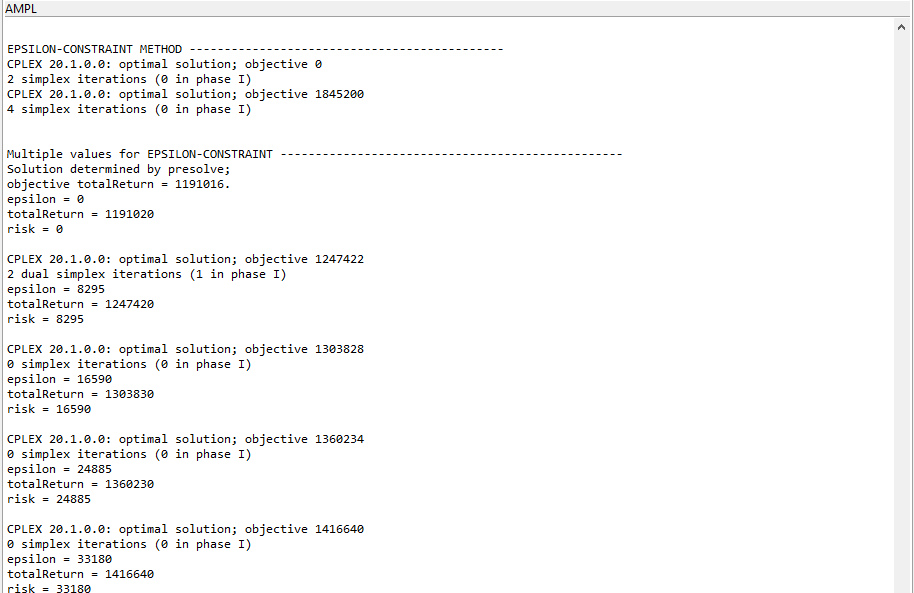
\includegraphics[width = .9\textwidth]{output1aiiii.png}

We include the text output generated from this exercise for completeness.

{\tiny \VerbatimInput{titanParetoEps.txt}}


\end{enumerate}
\item Pareto Front From $\epsilon$-Constraint


 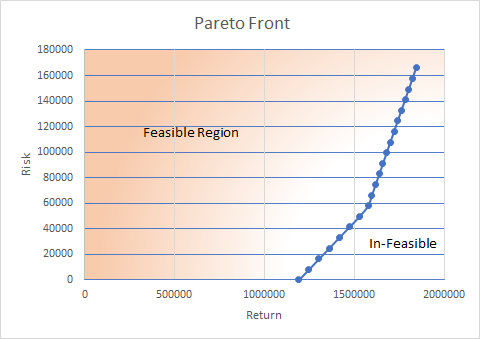
\includegraphics[width = .9\textwidth]{output1b.png}

Above we see the expression of the Pareto Front utilizing the data generated from the $\epsilon$- constraint method.  As we change the maximum allowed risk, we see the return on investment increase.  Anything to the left of our front will belong in the feasible set and everything to the right is not possible to achieve as we trade risk for greater returns.  We see an interesting feature of a corner where the risk to return slope becomes much steeper.  This shows that we will have to incur more risk to achieve more returns.

\item To discuss how the portfolio changes across time, we first examine the investments based on the risk/profit trade off.  We display the data here again for completeness


{\tiny \VerbatimInput{titanParetoEps.txt}}

We notice that the $B$, $C$, and $D$ investments are never used.  We note that as risk tolerance increases, more money is first invested into account $E$ and then into account $A$.  In the maximum return scenario, everything is invested in each of these accounts.  Let's visualize the trade-off by examining these two accounts.

  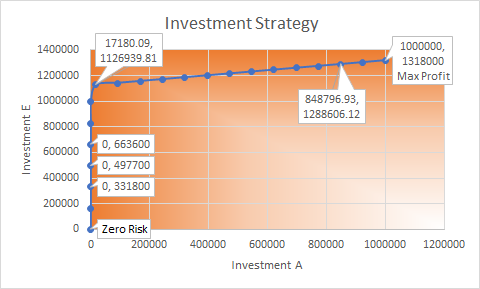
\includegraphics[width = .9\textwidth]{output1c.png}

Again we notice the corner.  This is not a coincidence as this corner occurs at $\epsilon = 7$ in both graphs.  We included a few data call outs to help illustrate the points represented in the graph.  We also believe that we did not need to include investments in the bank as banking is boring and provides no risk and little reward even though all values of $\epsilon$ use the bank at some point.
\end{enumerate}
\end{enumerate}



\end{document}
